% =====================================================================
% OpenSUN3D @ ECCV 2026 — archival proceedings track (8 pages, double-blind).
% SCAFFOLD ONLY. For the real submission, open the OFFICIAL ECCV 2026 author kit
% on Overleaf and paste these sections in (the kit sets the exact font + review
% line numbers; using another template risks desk-rejection):
%   https://www.overleaf.com/latex/templates/template-and-author-guidelines-for-eccv-submission/gycdswmdkkyv
% This file uses the LNCS base class (what ECCV is built on) so the content is
% structured correctly; it still needs (a) the official kit, (b) trimming to 8
% pages per docs/opensun3d_submission_plan.md, and (c) the n~=30 numbers + figures.
% =====================================================================
\documentclass[runningheads]{llncs}

\usepackage{booktabs}
\usepackage{graphicx}
\usepackage{amsmath}
\usepackage{amssymb}
\usepackage{multirow}
\usepackage[hidelinks]{hyperref}

% Placeholder marker for results pending the ~30-scene expansion run.
\newcommand{\todo}[1]{\textbf{[TODO: #1]}}

\begin{document}

\title{Open-Vocabulary 3D Scene Graphs from Sparse RGB Views:\\
Duplicate-Aware Fusion and a De-Circularized Benchmark}

% Double-blind: no authors / affiliations / repo links in the submitted version.
\author{Anonymous}
\institute{Anonymous}

\maketitle

\begin{abstract}
We present a sparse-view pipeline for constructing language-grounded 3D scene graphs
from casually captured RGB images. Feed-forward geometry models can now predict
cameras, depth, and world-point maps without per-scene optimization, while 2D
foundation models provide class-agnostic masks and open-vocabulary descriptors.
However, these outputs remain view-local: they do not directly identify persistent
objects, expose uncertain geometric evidence, or produce relation-bearing scene
structure. Our method bridges this gap by lifting SAM proposals into VGGT world-point
maps, attaching CLIP and DINOv2 descriptors, scoring lifted candidates with confidence
and compactness uncertainty, fusing cross-view candidates into object nodes, and
exporting open-vocabulary labels and spatial relations. The graph representation keeps
symbolic predictions together with source views, proposal support, 3D point samples,
and uncertainty values, making the output inspectable and reviewable. We evaluate the
pipeline on a five-sequence TUM RGB-D sparse-view benchmark with 20 runs across 3, 5,
8, and 10 input views. Averaged over scenes, moving from 3 to 10 views increases lifted
proposals from 54.0 to 173.6, fused objects from 31.8 to 72.2, multi-view objects from
11.8 to 28.2, and inferred relations from 585.2 to 2104.0. Against checked references
initialized from the 10-view graphs, non-reference object-label F1 improves from 0.622
to 0.914 and relation-triplet F1 from 0.434 to 0.799 between 3 and 8 views. These
reference-consistency scores measure sparse-view recovery rather than dense-scene
recognition accuracy, establishing a reproducible graph construction baseline and a
concrete path from predicted graphs to object-relation review.

\keywords{3D scene graphs \and sparse views \and open-vocabulary detection \and
evaluation methodology \and benchmark \and duplicate-aware fusion}
\end{abstract}

% NOTE: trim each \input to hit 8 pages (excl. references). Move the full IoU sweep,
% the full per-class table, and the weight-sweep table to an appendix/supplementary;
% consolidate the five result tables to two in the main body (see submission plan).
\section{Introduction}

\begin{figure}[t]
\centering

\includegraphics[width=0.72\linewidth]{fig_teaser.png}
\caption{From a handful of RGB views to an open-vocabulary 3D scene graph. \textbf{Left:} three input
frames (TUM \texttt{freiburg3\_long\_office\_household}). \textbf{Right:} frozen-model detections lifted
into VGGT world-point geometry and fused across views into labeled 3D object nodes (colored markers),
with all heavy models frozen and no per-scene optimization. Best viewed in color.}
\label{fig:teaser}
\end{figure}


Reconstructing a scene and explaining a scene differ. Feed-forward geometry models
recover camera motion, depth, and point maps from a few
images~\cite{wang2024dust3r,leroy2024mast3r,wang2025vggt}, and 2D foundation models give
open-vocabulary detections, masks, and
descriptors~\cite{minderer2023owlv2,radford2021clip,kirillov2023segment,oquab2023dinov2}. Many
applications instead need object-level structure: which pixels across views belong to the same
object, where it sits in 3D, and how it relates to others, so a robot can act on
``the monitor is on the desk'' rather than a raw point cloud. These components do not provide
this alone, and the gap is widest for a handful of casual RGB views rather than a
calibrated RGB-D stream or prebuilt map.

We build the scene graph by fusing lifted 2D detections, keeping every heavy model frozen with no
per-scene optimization. VGGT world-point maps act as a 2D-to-3D lookup, an open-vocabulary detector
proposes labeled object boxes, and we lift and fuse these across views into an object--relation graph
(Figure~\ref{fig:teaser}). Fixed perception isolates the graph-building stage for ablation and
places us in a lower-input regime than open-vocabulary 3D systems assuming posed RGB-D video
or a dense map~\cite{gu2024conceptgraphs,jatavallabhula2023conceptfusion}.

A central lesson of this work concerns evaluation. An earlier version graded
predicted graphs against a reference seeded from the model's own dense-view output, which is circular: a
method reproducing its ten-view graph scores $1.0$ at the reference view by construction, rewarding
agreement with the model rather than the scene. Rebuilding the
reference from the frames themselves changes two conclusions. First, a mask-plus-CLIP front-end recovers
almost no real objects; on a desk scene it returns ``floor'', ``curtain'', and ``bed''
instead of the present monitors and keyboard, whereas a genuine open-vocabulary detector
(OWLv2) reads the actual objects. Second, an uncertainty-aware fusion gate that looked promising
under the old protocol gives no improvement once labels are real, across a full weight sweep.
With honest labels, the dominant error is over-counting: one physical object survives
fusion as several same-label nodes (Figure~\ref{fig:dedup3d}). A one-line merge of same-label nodes
with overlapping 3D boxes removes most of it, the only variant whose accuracy improves with views.

We test these on 28 TUM RGB-D sequences~\cite{sturm2012tumrgbd} at $3/5/8/10$ views, against a
reference authored from the frames (5 scenes human-verified, 23 drafted in two passes). Duplicate-aware
fusion improves object-label F1 over the graph-fusion baseline by $0.06$ to $0.12$ and wins on $22$ to
$27$ of the $28$ scenes ($p<0.001$), while the uncertainty gate is consistently worse. We make four
contributions. \textbf{(1)}~A detector-grounded open-vocabulary scene-graph system for sparse views that
keeps OWLv2 and VGGT frozen with no per-scene optimization, recovering real
objects a mask-plus-CLIP front-end misses. \textbf{(2)}~Duplicate-aware cross-view fusion, a single
post-fusion merge of same-label nodes with overlapping 3D boxes that targets over-counting and
is the only variant whose accuracy improves with more views. \textbf{(3)}~An independent,
de-circularized benchmark on TUM RGB-D, showing how a prediction-seeded reference inflates scores
while an independently authored one removes the effect. \textbf{(4)}~A negative result on
uncertainty-aware fusion, with analysis: the gate raises recall but
over-splits, costing more precision than it gains, so merging helps.
\section{Related Work}
\label{sec:related_work}

\paragraph{Feed-forward sparse-view geometry.}
Multi-view reconstruction and SLAM classically rely on correspondence, triangulation,
bundle adjustment, and calibrated or densely overlapping observations. COLMAP remains a
standard reference for incremental structure from motion~\cite{schonberger2016sfm},
while ORB-SLAM3 demonstrates the strength of optimized visual and visual-inertial SLAM
for coherent streams~\cite{campos2021orbslam3}. Feed-forward 3D models reduce this
dependence on per-scene optimization. DUSt3R casts reconstruction as point-map
prediction from unconstrained images~\cite{wang2024dust3r}; MASt3R adds 3D-aware dense
matching~\cite{leroy2024mast3r}; and VGGT predicts camera parameters, depth, point
maps, confidence, and tracks from one or many views~\cite{wang2025vggt}. These models
provide the geometric substrate for our work. We use VGGT as a frozen source of
pixel-aligned 3D evidence, but our output is not a reconstruction: it is an
object-relation graph grounded in that geometry.

\paragraph{Open-vocabulary 2D and 3D semantics.}
Our 2D proposal and feature stack builds on SAM for class-agnostic masks,
CLIP for language-aligned visual embeddings, and DINOv2 for robust self-supervised
appearance descriptors~\cite{kirillov2023segment,radford2021clip,oquab2023dinov2}.
In 3D, open-vocabulary scene understanding has been explored by lifting, distilling,
or optimizing foundation-model features into point clouds, maps, masks, and neural
scene representations. NeRF introduced continuous radiance fields for view
synthesis~\cite{mildenhall2020nerf}; LERF embeds language features into radiance
fields for open-ended 3D queries~\cite{kerr2023lerf}; and 3D Gaussian Splatting has
become a common explicit substrate for fast scene representations~\cite{kerbl2023gaussian}.
OpenScene learns open-vocabulary point features aligned with image and text
embeddings~\cite{peng2023openscene}; ConceptFusion builds queryable 3D maps by fusing
pixel-aligned open-set features~\cite{jatavallabhula2023conceptfusion}; OpenMask3D
aggregates CLIP features over class-agnostic 3D instance masks~\cite{takmaz2023openmask3d};
CUA-O3D studies cross-modal and uncertainty-aware agglomeration for open-vocabulary
3D scene understanding~\cite{li2025cuao3d}; and OpenSplat3D performs open-vocabulary
3D instance segmentation in a Gaussian Splatting representation~\cite{piekenbrinck2025opensplat3d}.
These methods motivate foundation-feature fusion in 3D. Our contribution is
complementary: we construct explicit object-relation graphs from sparse RGB views
without assuming a completed 3D map or optimizing a per-scene radiance field.

\paragraph{3D scene graphs.}
3D scene graphs organize object instances and their relationships as structured
representations for reasoning about scenes. Early work proposed unified graphs spanning
objects, spaces, cameras, and semantic or spatial relationships~\cite{armeni2019scenegraph}.
3DSSG introduced a large-scale dataset and learned prediction framework for semantic
scene graphs from 3D indoor reconstructions~\cite{wald2020threedssg}. RGB-D resources
such as ScanNet further show the value of richly annotated reconstructed scenes for
indoor understanding~\cite{dai2017scannet}. ConceptGraphs is closest to our output
space: it builds open-vocabulary 3D scene graphs from posed RGB-D sequences by fusing
2D foundation-model outputs into object nodes and relations~\cite{gu2024conceptgraphs}.
We share the object-relation motivation, but relax the input assumption. Instead of
requiring a depth stream, posed RGB-D map, or completed 3D reconstruction, we lift
sparse-view 2D proposals through feed-forward VGGT point maps and build object
identities through cross-view geometric and semantic fusion.

\section{Method}
\label{sec:method}

\subsection{Problem Setup}

Given a sparse set of RGB views $\mathcal{I}=\{I_1,\ldots,I_V\}$, the goal is to
produce a 3D scene graph $\mathcal{G}=(\mathcal{O},\mathcal{R})$. Each object node
$o_i \in \mathcal{O}$ stores a 3D point set, centroid, open-vocabulary label, view
support, feature descriptor, source proposals, and uncertainty. Each relation edge
$r_{ij} \in \mathcal{R}$ stores a spatial predicate between two object nodes. The
method does not assume depth images, externally supplied camera poses, or a prebuilt
mesh. It instead derives geometry, object proposals, and proposal descriptors from
frozen feed-forward models, then performs object-level fusion and relation inference
over the resulting evidence. Figure~\ref{fig:method_pipeline} summarizes the complete
data flow.

\begin{figure}[t]
\centering
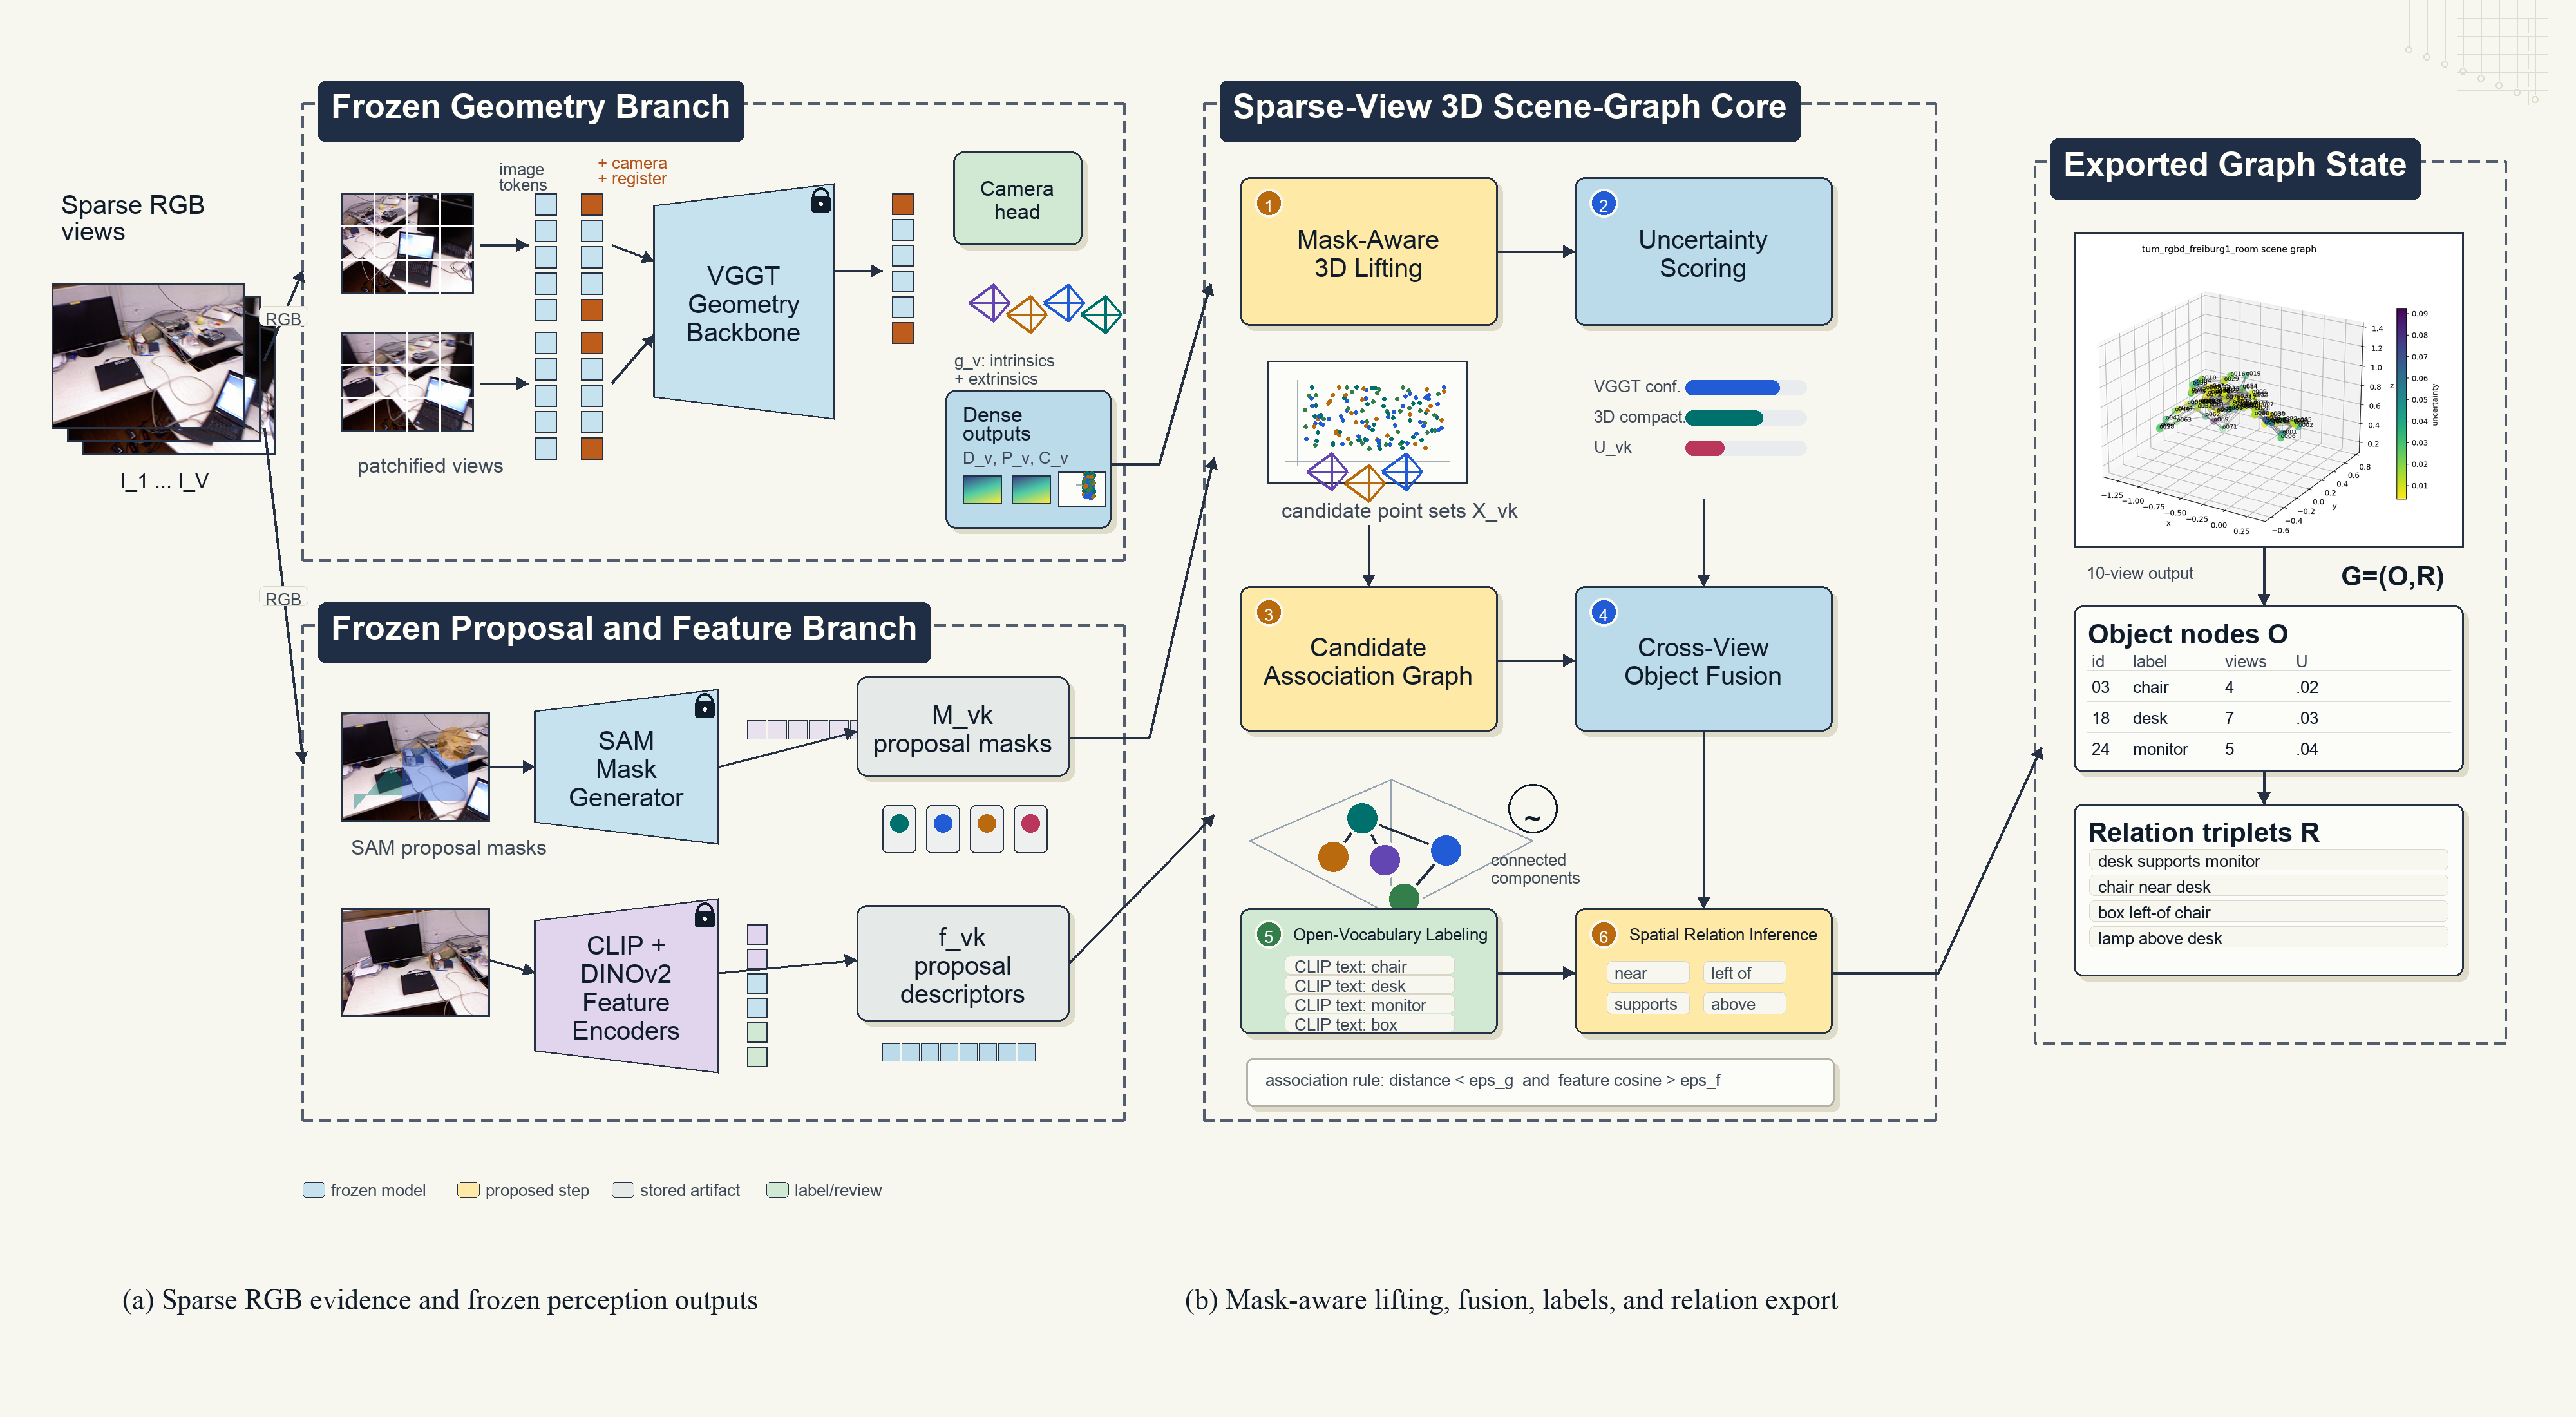
\includegraphics[width=0.98\textwidth]{figures/method_pipeline}
\caption{Architecture of the proposed sparse-view 3D scene graph system. The figure
shows the actual artifacts passed between stages: sparse RGB frames, patch and camera
tokens, frozen VGGT camera/depth/world-point/confidence outputs, SAM masks,
CLIP+DINOv2 proposal descriptors, lifted 3D candidate point sets, uncertainty scores,
association edges, fused objects, open-vocabulary labels, relation predicates, and the
exported scene graph $\mathcal{G}=(\mathcal{O},\mathcal{R})$.}
\label{fig:method_pipeline}
\end{figure}

\subsection{Overview}

The pipeline has five stages. First, VGGT predicts camera parameters, depth maps,
world-point maps, and confidence maps for the selected sparse views. Second, SAM
generates view-local object proposals, and CLIP+DINOv2 descriptors are extracted for
each proposal. Third, every proposal mask is lifted into the VGGT world-point map to
form a 3D candidate object fragment with a confidence and compactness uncertainty
score. Fourth, candidates from different views are connected when they are close in 3D
and sufficiently similar in descriptor space; connected components become fused object
nodes. Fifth, fused nodes are assigned open-vocabulary labels and connected by spatial
relation predicates. The output graph keeps the predicted labels and relations together
with the evidence used to produce them, so the graph can be inspected or converted into
annotation review packets.

\subsection{Sparse-View Geometry}

We run VGGT on the selected sparse views and save camera intrinsics, extrinsics, depth
maps, world-point maps, and confidence maps~\cite{wang2025vggt}. The world-point map
for each view acts as a 2D-to-3D lookup table. This is the key simplification: object
proposals can be lifted directly from image coordinates into a common 3D frame without
first reconstructing a mesh, running bundle adjustment, or optimizing a radiance-field
or Gaussian Splatting representation~\cite{schonberger2016sfm,mildenhall2020nerf,kerbl2023gaussian}.
For view $v$, we denote the world-point map by $P_v(u) \in \mathbb{R}^3$ and the
corresponding confidence map by $C_v(u)$ at image coordinate $u$.

\subsection{2D Proposals and Features}

SAM produces class-agnostic masks for each view~\cite{kirillov2023segment}. For
proposal $k$ in view $v$, we store the bounding box, confidence score, RLE mask, and
visual descriptors. CLIP supplies the language-aligned component, while DINOv2 adds a
complementary self-supervised appearance signal~\cite{radford2021clip,oquab2023dinov2}.
When both descriptors are available, the normalized vectors are concatenated and
renormalized:
\begin{equation}
    f_{v,k} =
    \frac{[\hat{f}^{\mathrm{CLIP}}_{v,k};\hat{f}^{\mathrm{DINO}}_{v,k}]}
    {\|[\hat{f}^{\mathrm{CLIP}}_{v,k};\hat{f}^{\mathrm{DINO}}_{v,k}]\|_2}.
\end{equation}
If one descriptor is unavailable, the valid normalized descriptor is retained. This
keeps the fusion stage usable across proposal files with different feature backends.

\subsection{Mask-Aware 3D Lifting}

Each 2D proposal mask $M_{v,k}$ is resized to the VGGT geometry resolution. The mask
selects world points from the corresponding view, while non-finite points and points
below the confidence threshold $\tau_c$ are discarded:
\begin{equation}
    X_{v,k} = \{P_v(u) \mid u \in M_{v,k},\, C_v(u) \geq \tau_c\}.
\end{equation}
Proposals with no valid lifted points are rejected. The remaining candidate node
stores a sampled 3D point set $X_{v,k}$, centroid $\mu_{v,k}$, 3D bounding box,
proposal metadata, visual feature $f_{v,k}$, and an uncertainty score. The uncertainty
combines VGGT point confidence with the spatial compactness of the lifted 3D points:
\begin{equation}
    U_{v,k} = \lambda(1-\bar{C}_{v,k}) + (1-\lambda)\,
    \mathrm{clip}\left(\frac{\sigma(X_{v,k})}{s_0},0,1\right),
\end{equation}
where $\bar{C}_{v,k}$ is the mean confidence of the selected points and
$\sigma(X_{v,k})$ summarizes spread around the median 3D point. In the implementation,
$\lambda=0.7$ and $s_0=1$. The score is not treated as an oracle; it is exported with
each node and used to prioritize ambiguous objects for later inspection.

\subsection{Graph Fusion}

Candidate nodes are fused by building an association graph over lifted proposals. We
disallow same-view association edges by default, so a component represents cross-view
object support rather than grouping proposals from a single image. An edge connects two
candidates when their centroids are close in 3D and, when valid descriptors exist,
their cosine similarity exceeds a feature threshold:
\begin{equation}
    \|\mu_a-\mu_b\|_2 \leq \epsilon_g
    \quad\mathrm{and}\quad
    \cos(f_a,f_b) \geq \epsilon_f.
\end{equation}
The feature condition is omitted for candidates without valid descriptors. Connected
components define fused object identities. For each component, points are pooled and
sampled, descriptors are averaged and renormalized, and the uncertainty is averaged
then reduced according to the number of supporting views. This separates view-local
evidence from object identity while preserving the proposal provenance needed for
debugging and annotation.

\subsection{Relation Inference and Labeling}

Spatial relations are inferred from fused centroids using distance and relative
coordinate rules. The relation vocabulary includes \emph{near}, \emph{left\_of},
\emph{right\_of}, \emph{above}, \emph{below}, \emph{in\_front\_of}, and
\emph{behind}. A near relation is emitted for object pairs within a distance threshold;
otherwise the vertical displacement or dominant horizontal coordinate determines the
directional predicate, with an optional maximum relation distance limiting very distant
pairs. For language grounding, fused nodes are labeled by comparing averaged visual
descriptors against CLIP text embeddings from an open-vocabulary label
set~\cite{radford2021clip}. The exported graph preserves both symbolic fields and
numeric support data, allowing the same object identities, point sets, labels, and
uncertainty values to be reused by manual review or future learned relation heads.

\section{Experiments}
\label{sec:experiments}

We study two questions: what actually helps when building open-vocabulary 3D scene
graphs from a handful of RGB views, and how to measure it honestly --- the second
matters because the system was originally reported as a sparse-view win for
uncertainty-aware fusion, an artifact of a circular evaluation. We describe the
benchmark (Sec.~\ref{sec:exp_scenes}), its de-circularized reference
(Sec.~\ref{sec:exp_reference}), and the variants and metric
(Sec.~\ref{sec:exp_variants}--\ref{sec:exp_metric}) before the results
(Section~\ref{sec:results}).

\subsection{Benchmark Scenes and Sparse-View Protocol}
\label{sec:exp_scenes}

We benchmark on public TUM RGB-D indoor sequences~\cite{sturm2012tumrgbd}. The
benchmark spans \textbf{28 object-rich sequences} across \texttt{freiburg1}--\texttt{freiburg3}:
the five paper-subset scenes in Table~\ref{tab:tum_rgbd_paper_subset_plan} (which carry the
human-verified gold reference) plus 23 additional sequences; the full list is in
\texttt{tum\_rgbd\_expanded.json}. Each sequence contributes ten
selected RGB frames (stride~10). Although the source benchmark is RGB-D, our
pipeline consumes only RGB; we use this dataset because it provides public,
recognizable indoor scenes with reproducible sequence identifiers.

\begin{table}[t]
\centering
\caption{TUM RGB-D sequences prepared for sparse-view benchmarking. Each sequence contains 10 selected RGB frames and is evaluated with 3, 5, 8, and 10 input views.}
\label{tab:tum_rgbd_paper_subset_plan}
\small
\resizebox{\linewidth}{!}{%
\begin{tabular}{l l r l}
\hline
Scene ID & Source sequence & Frames & View counts \\
\hline
\texttt{tum\_rgbd\_freiburg1\_room} & \texttt{freiburg1\_room} & 10 & 3/5/8/10 \\
\texttt{tum\_rgbd\_freiburg1\_desk} & \texttt{freiburg1\_desk} & 10 & 3/5/8/10 \\
\texttt{tum\_rgbd\_freiburg1\_desk2} & \texttt{freiburg1\_desk2} & 10 & 3/5/8/10 \\
\texttt{tum\_rgbd\_freiburg2\_xyz} & \texttt{freiburg2\_xyz} & 10 & 3/5/8/10 \\
\texttt{tum\_rgbd\_freiburg3\_long\_office\_household} & \texttt{freiburg3\_long\_office\_household} & 10 & 3/5/8/10 \\
\hline
\end{tabular}
}
\end{table}


For each scene we evaluate $N \in \{3, 5, 8, 10\}$ input views (a $28\times4$ matrix,
112 graphs per variant), each run end-to-end along an identical code path --- the
pipeline of Section~\ref{sec:method}, driven by
\texttt{run\_owlv2\_benchmark.sh}. Reporting accuracy as a function of $N$
reads off sparse-view behavior directly rather than a single dense-view number.

\subsection{An Independently-Authored Reference}
\label{sec:exp_reference}

\begin{figure}[t]
\centering
\begin{tikzpicture}[font=\small,
   pbox/.style={fxbox, minimum width=26mm},
   tiny/.style={font=\scriptsize}]
% ================= LEFT: circular (prior) =================
\begin{scope}
  \node[font=\footnotesize\bfseries, color=cWarn] (t1) at (0,2.45) {Prior pseudo-reference (circular)};
  \node[pbox, draw=cWarn, fill=cWarnFill] (src1) at (0,1.45) {Model 10-view\\\textsc{graph-fusion} output};
  \node[pbox, draw=cWarn, fill=cWarnFill, dashed] (ref1) at (0,0.05) {Pseudo-reference};
  \node[pbox] (pred1) at (0,-1.45) {Variant predictions\\{\scriptsize 3 / 5 / 8 / 10 views}};
  \node[circle, draw=cInk!70, fill=white, inner sep=1.4pt, font=\scriptsize] (cmp1) at (2.55,-0.70) {F1};
  \draw[flow, draw=cWarn] (src1) -- node[right=1pt,tiny,color=cWarn]{copied as} (ref1);
  \draw[flow] (ref1.east) -| (cmp1.north);
  \draw[flow] (pred1.east) -| (cmp1.south);
  % the loop: predictions come from the same model that defined the reference
  \draw[draw=cWarn, densely dashed, -{Stealth[length=2mm]}, line width=0.7pt]
       (pred1.west) to[out=180,in=180,looseness=1.5] node[left,tiny,color=cWarn,align=right]{same\\model} (src1.west);
  \node[tiny, color=cWarn, align=center, text width=42mm] at (0.7,-2.7)
    {\textbf{Inflated:} \textsc{graph-fusion}$=\!1.0$ at v10 \emph{by construction}; a variant that splits more is \emph{rewarded}};
\end{scope}
% divider
\draw[gray!45, densely dashed] (3.95,2.7) -- (3.95,-3.2);
% ================= RIGHT: independent (ours) =================
\begin{scope}[xshift=6.2cm]
  \node[font=\footnotesize\bfseries, color=cOk] (t2) at (0,2.45) {Independent reference (ours)};
  \node[pbox, draw=cOk, fill=cOkFill] (src2) at (0,1.45) {Raw RGB frames\\$+$ human, 2-pass};
  \node[pbox, draw=cOk, fill=cOkFill] (ref2) at (0,0.05) {Independent reference};
  \node[pbox] (pred2) at (0,-1.45) {Variant predictions\\{\scriptsize 3 / 5 / 8 / 10 views}};
  \node[circle, draw=cInk!70, fill=white, inner sep=1.4pt, font=\scriptsize] (cmp2) at (2.55,-0.70) {F1};
  \draw[flow, draw=cOk] (src2) -- node[right=1pt,tiny,color=cOk]{authored from} (ref2);
  \draw[flow] (ref2.east) -| (cmp2.north);
  \draw[flow] (pred2.east) -| (cmp2.south);
  \node[tiny, color=cOk, align=center, text width=44mm] at (0.7,-2.7)
    {\textbf{Honest:} object count fixed independently; over-splitting \emph{penalized} $\Rightarrow$ uncertainty reverses, dedup wins};
\end{scope}
\end{tikzpicture}
\caption{De-circularizing the evaluation. \textbf{Left:} the earlier protocol seeded the reference
from the model's own ten-view \textsc{graph-fusion} prediction, so that variant scores $1.0$ at ten
views \emph{by construction}, and a variant that keeps more proposals unmerged (the uncertainty gate)
is rewarded for reproducing the reference's own fragments---an apparent sparse-view win.
\textbf{Right:} our reference is authored from the raw RGB frames, independently of any model output.
The true object count is fixed, over-splitting is penalized, and both findings emerge: the uncertainty
gate reverses to a loss and duplicate-aware fusion wins.}
\label{fig:decirc}
\end{figure}


The central evaluation problem in this setting is that there is no
ground-truth open-vocabulary object inventory for TUM RGB-D scenes, so a
reference must be constructed. The tempting shortcut --- and the one the
original version of this work took --- is to seed the reference from the
system's own dense-view prediction (the 10-view graph) and then lightly check
it. We argue this is unsound and replace it with a reference authored
\emph{from the frames}.

\paragraph{Why a prediction-seeded reference is circular.}
Seeding the reference from a variant's own 10-view output (Figure~\ref{fig:decirc}, left) makes that
variant score $1.0$ at ten views \emph{by construction} and grades every sparser run on how faithfully
it reproduces the same splitting pattern rather than agreement with the scene --- so a method that
keeps more proposals unmerged is rewarded for reproducing the reference's own fragments. The
quantitative artifacts this produced (the apparent uncertainty win, the dense-view ceiling) are in
Section~\ref{subsec:decirc}.

\paragraph{Construction of the independent reference.}
Our reference is, for each scene, an object multiset enumerated only from the ten raw RGB frames,
independent of the detection/descriptor/geometry/fusion stack under test. Each scene is drafted once
and re-examined in a second, adversarial pass that seeks missed or spurious objects. The five
paper-subset scenes are additionally \textbf{human-verified} against the frames (the gold core,
\texttt{independent\_labels.json}); the other 23 use the two-pass draft \emph{without} verification
(\texttt{independent\_labels\_expanded.json}) as scale corroboration, and both findings also hold on
the gold five alone. Because the reference fixes the object inventory without reference to any model
output, no variant can score $1.0$ at ten views and over-splitting is penalized. It is a scene-level
multiset over all ten frames, so sparse-view predictions are recall-limited against it --- depressing
absolute F1 uniformly across variants and leaving the comparison fair.

\subsection{Variants Compared}
\label{sec:exp_variants}

We hold the front-end (OWLv2 detections lifted by VGGT geometry) and the
reference fixed, and compare seven variants that differ only in how per-view
detections become 3D nodes and how those nodes are fused across views:

\begin{itemize}
  \item \textbf{2d-only} --- per-view OWLv2 labels pooled without 3D lifting or
        cross-view fusion (an image-level upper reference on labels alone).
  \item \textbf{geometry-only} --- detections lifted to 3D via VGGT and pooled,
        with no semantic cross-view association.
  \item \textbf{semantic-lifting} --- detections lifted and associated by
        appearance descriptors without the geometric fusion gate.
  \item \textbf{fixed-shrink (uninformed control)} --- the fusion gate is
        modulated by a fixed, scene-agnostic shrink factor; an
        uncertainty-blind control that isolates whether the
        \emph{uncertainty signal}, rather than merely the act of tightening the
        gate, carries any benefit.
  \item \textbf{graph-fusion (baseline)} --- the standard cross-view fusion of
        Section~\ref{sec:method} with no uncertainty modulation and no
        duplicate handling.
  \item \textbf{proposed (uncertainty)} --- graph-fusion with the
        rank-normalized uncertainty-aware merge gate (default weight
        $w{=}0.3$); evaluated as an ablation rather than the headline method,
        and additionally swept over $w \in \{0.1, 0.2, 0.3, 0.5, 0.8\}$.
  \item \textbf{graph-fusion-dedup (ours)} --- graph-fusion followed by a single
        post-fusion duplicate-instance merge: same-label fused nodes whose
        axis-aligned 3D boxes overlap (IoU~$>\tau$, default $\tau{=}0.1$) are
        unioned and re-fused (\texttt{merge\_duplicate\_instances} in
        \texttt{graph\_builder.py}). This targets the measured over-counting
        failure (Section~\ref{sec:results}) and is the opposite move from the
        uncertainty gate, which \emph{tightens} merging.
\end{itemize}

The pairing is deliberate: \emph{fixed-shrink} versus \emph{proposed} asks
whether the uncertainty signal is informative beyond an uninformed gate
adjustment, and \emph{graph-fusion} versus \emph{graph-fusion-dedup} asks
whether merging \emph{more} (rather than less) is the productive direction.

\subsection{Metric}
\label{sec:exp_metric}

Our primary metric is \texttt{object\_label\_f1}: the multiset precision,
recall, and F1 of fused-node labels against the independent reference multiset,
averaged over the 28 scenes (5 human-verified, 23 two-pass VLM-drafted). Treating
labels as a multiset (rather than a set) makes the metric sensitive to
over-counting --- a scene with one physical monitor reported as four fused monitor
nodes is penalized on precision --- which is exactly the failure mode the reframed
contribution targets. Per-scene wins/losses are reported alongside the means, with
significance from a two-sided sign-test. Evaluation is run by
\texttt{evaluate\_sparse\_view\_annotations.py} and aggregated by
\texttt{aggregate\_variant\_f1.py}; raw per-(scene, $N$, variant) scores
are in \texttt{variant\_independent\_metrics.csv}.

\subsection{Implementation Details}
\label{sec:exp_impl}

All heavy models are frozen and run off-the-shelf; there is no per-scene
optimization or fine-tuning. The open-vocabulary detector is OWLv2
(\texttt{google/owlv2-base-patch16-ensemble})~\cite{minderer2023owlv2}, the
successor to OWL-ViT~\cite{minderer2022owlvit}, with a detection score threshold
of $0.2$ and per-class non-maximum suppression at IoU~$0.5$; detection boxes
prompt SAM~\cite{kirillov2023segment} for masks. 3D geometry is the feed-forward
VGGT transformer~\cite{wang2025vggt}, consuming RGB frames only. Appearance
descriptors for cross-view association use CLIP~\cite{radford2021clip} and
DINOv2~\cite{oquab2023dinov2}. VGGT geometry runs on GPU; detection, lifting,
fusion, and evaluation run on CPU. We fix all thresholds across scenes and view
counts (no per-scene tuning), and the duplicate-aware merge uses a single global
IoU threshold $\tau{=}0.1$ that we show is robust across $\tau \in [0, 0.2]$
(Section~\ref{sec:results}).

\subsection{Static and dynamic subsets}
\label{sec:exp_expansion}

Six of the 28 sequences are \emph{dynamic} (a moving person: \texttt{desk\_with\_person},
\texttt{sitting\_*}, \texttt{walking\_*}), which violates VGGT's static multi-view assumption; the
other 22 are static. We report the two as separate subsets and analyze the duplicate-aware gain on
each with the results (Section~\ref{subsec:dedup}).

\section{Results}
\label{sec:results}

\subsection{TUM RGB-D Validation}

Table~\ref{tab:tum_rgbd_sparse_view} summarizes the 3/5/8/10-view validation run on
\texttt{freiburg1\_room}. The run exercises the complete path from RGB frames to VGGT
geometry, SAM proposals, CLIP+DINOv2 descriptors, object fusion, open-vocabulary
labels, and spatial relations. As the view count increases, lifted proposals increase
from 58 to 198, multi-view object support increases from 18 to 28 nodes, and mean
uncertainty decreases from 0.014525 to 0.011513. This establishes the expected
single-scene behavior before moving to the five-sequence benchmark.

\begin{table}[t]
\centering
\caption{Sparse-view curve on TUM RGB-D \texttt{freiburg1\_room}.}
\label{tab:tum_rgbd_sparse_view}
\small
\resizebox{\linewidth}{!}{%
\begin{tabular}{rrrrrrr}
\toprule
Views & Candidates & Objects & Multi-view & Relations & Uncertainty & MV Ratio \\
\midrule
3 & 58 & 27 & 18 & 466 & 0.014525 & 0.666667 \\
5 & 98 & 32 & 24 & 628 & 0.014585 & 0.750000 \\
8 & 158 & 30 & 26 & 580 & 0.011999 & 0.866667 \\
10 & 198 & 32 & 28 & 636 & 0.011513 & 0.875000 \\
\bottomrule
\end{tabular}
}
\end{table}


\subsection{Component Ablation}

Table~\ref{tab:local_ablation} compares local variants on the development scene. With
the number of lifted candidates fixed, moving from geometry-only OpenCV proposals to
feature-aware fusion lowers mean uncertainty and increases multi-view support. Replacing
OpenCV proposals with SAM masks produces more fused objects and relations, and adding
DINOv2 to CLIP yields the richest graph among the tested variants. This ablation is
local rather than a full benchmark, but it supports the design choice of combining
class-agnostic mask proposals with complementary language-aligned and self-supervised
features.

\begin{table}[t]
\centering
\caption{Development-scene component ablation on a four-view example.}
\label{tab:local_ablation}
\resizebox{\linewidth}{!}{%
\begin{tabular}{lllrrrrr}
\toprule
Variant & Proposals & Features & Candidates & Objects & Multi-view & Relations & Uncertainty \\
\midrule
OpenCV geometry-only & OpenCV & none & 80 & 14 & 9 & 100 & 0.039071 \\
OpenCV feature fusion & OpenCV & clip+handcrafted & 80 & 16 & 10 & 142 & 0.024012 \\
SAM semantic fusion & SAM & clip & 80 & 22 & 15 & 278 & 0.021765 \\
Full pipeline & SAM & clip+dinov2 & 80 & 33 & 17 & 618 & 0.021568 \\
\bottomrule
\end{tabular}
}
\end{table}


\subsection{Benchmark Results}

Table~\ref{tab:tum_rgbd_paper_subset_by_view} reports the five-sequence sparse-view
benchmark. It contains 20 runs: five scenes evaluated at 3, 5, 8, and 10 input views
with the same VGGT, SAM, CLIP+DINOv2, labeling, fusion, and relation inference code.
Averaged over scenes, increasing the view count from 3 to 10 raises lifted object
candidates from 54.0 to 173.6, fused object nodes from 31.8 to 72.2, multi-view object
nodes from 11.8 to 28.2, and inferred spatial relations from 585.2 to 2104.0. The
growth in multi-view nodes is important: additional views do not merely add isolated
proposals, but increase the number of objects supported by evidence from multiple
images. The structural counts measure graph coverage; label and relation consistency
are evaluated separately below.

\begin{table}[t]
\centering
\caption{Average sparse-view scene graph statistics over five TUM RGB-D sequences.}
\label{tab:tum_rgbd_paper_subset_by_view}
\small
\resizebox{\linewidth}{!}{%
\begin{tabular}{rrrrrrr}
\toprule
Views & Scenes & Candidates & Objects & Multi-view & Relations & Uncertainty \\
\midrule
3 & 5 & 54.00 & 31.80 & 11.80 & 585.20 & 0.026421 \\
5 & 5 & 88.60 & 42.80 & 16.80 & 912.80 & 0.035933 \\
8 & 5 & 140.20 & 61.40 & 24.20 & 1472.40 & 0.036613 \\
10 & 5 & 173.60 & 72.20 & 28.20 & 2104.00 & 0.034249 \\
\bottomrule
\end{tabular}
}
\end{table}


Table~\ref{tab:tum_rgbd_paper_subset_results} gives the per-scene breakdown. The full
run outputs are stored under
\texttt{results/benchmark\_tum\_rgbd\_paper\_subset/}; aggregate statistics are exported
to \texttt{sparse\_view\_scene\_graph\_summary.csv} and proxy metrics to
\texttt{sparse\_view\_scene\_graph\_metrics.csv}. Checked reference-consistency
metrics are exported to \texttt{sparse\_view\_checked\_metrics.csv}.

\begin{table}[t]
\centering
\caption{Per-scene sparse-view scene graph statistics on the TUM RGB-D benchmark subset.}
\label{tab:tum_rgbd_paper_subset_results}
\small
\resizebox{\linewidth}{!}{%
\begin{tabular}{lrrrrrr}
\toprule
Scene & Views & Candidates & Objects & Multi-view & Relations & Uncertainty \\
\midrule
freiburg1\_desk & 3 & 56 & 33 & 13 & 602 & 0.032715 \\
freiburg1\_desk & 5 & 93 & 44 & 16 & 752 & 0.031488 \\
freiburg1\_desk & 8 & 153 & 70 & 26 & 1314 & 0.037485 \\
freiburg1\_desk & 10 & 193 & 81 & 30 & 1718 & 0.044303 \\
freiburg1\_desk2 & 3 & 41 & 31 & 5 & 414 & 0.031997 \\
freiburg1\_desk2 & 5 & 66 & 42 & 14 & 694 & 0.040113 \\
freiburg1\_desk2 & 8 & 113 & 79 & 20 & 1602 & 0.042473 \\
freiburg1\_desk2 & 10 & 151 & 110 & 25 & 3564 & 0.038729 \\
freiburg1\_room & 3 & 57 & 41 & 10 & 1088 & 0.022612 \\
freiburg1\_room & 5 & 93 & 64 & 15 & 2100 & 0.024899 \\
freiburg1\_room & 8 & 134 & 76 & 25 & 2836 & 0.022970 \\
freiburg1\_room & 10 & 158 & 80 & 30 & 3192 & 0.021626 \\
freiburg2\_xyz & 3 & 56 & 31 & 14 & 484 & 0.022882 \\
freiburg2\_xyz & 5 & 91 & 33 & 19 & 518 & 0.022266 \\
freiburg2\_xyz & 8 & 144 & 42 & 24 & 840 & 0.025731 \\
freiburg2\_xyz & 10 & 169 & 47 & 26 & 1130 & 0.024507 \\
freiburg3\_long\_office\_household & 3 & 60 & 23 & 17 & 338 & 0.021901 \\
freiburg3\_long\_office\_household & 5 & 100 & 31 & 20 & 500 & 0.060900 \\
freiburg3\_long\_office\_household & 8 & 157 & 40 & 26 & 770 & 0.054405 \\
freiburg3\_long\_office\_household & 10 & 197 & 43 & 30 & 916 & 0.042079 \\
\bottomrule
\end{tabular}
}
\end{table}


\begin{figure}[t]
\centering
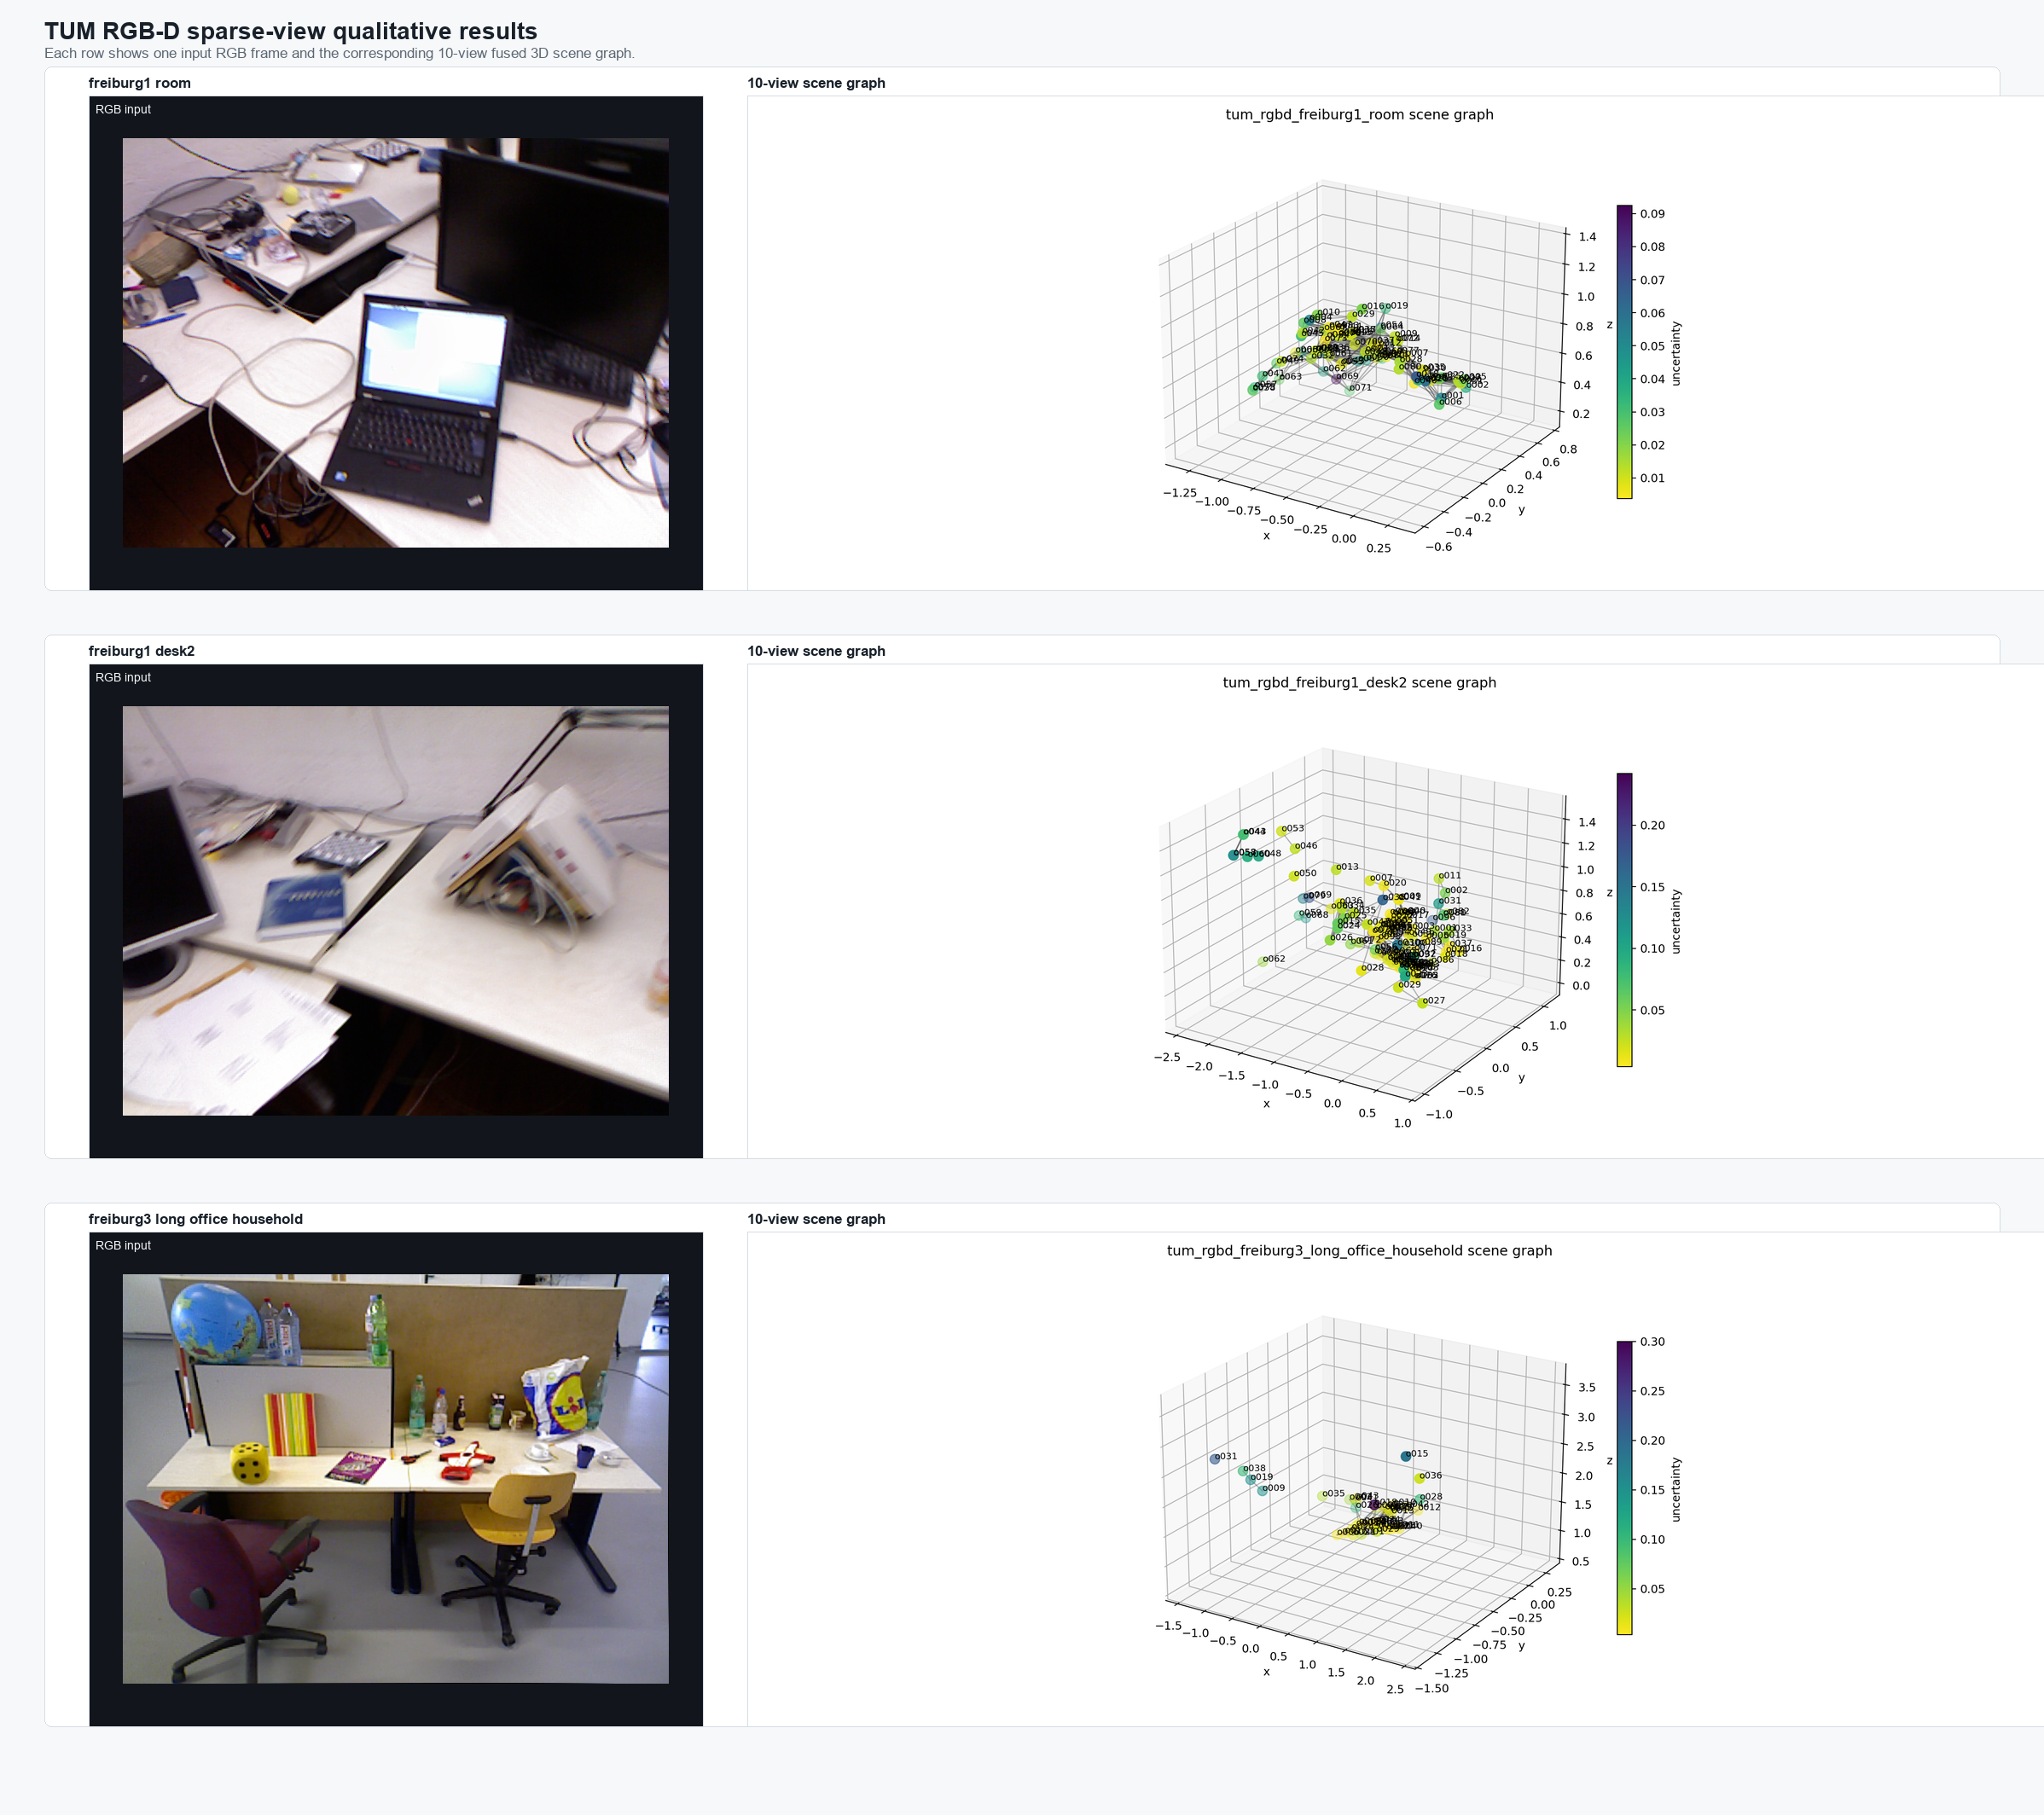
\includegraphics[width=0.98\textwidth]{figures/tum_rgbd_paper_subset_qualitative}
\caption{Qualitative examples from the TUM RGB-D benchmark subset. Each row shows one
input RGB frame and the corresponding 10-view fused 3D scene graph visualization. Node
colors encode uncertainty and edge overlays show inferred near relations.}
\label{fig:tum_rgbd_paper_subset_qualitative}
\end{figure}

Figure~\ref{fig:tum_rgbd_paper_subset_qualitative} shows representative qualitative
outputs from the benchmark. The examples show sparse RGB observations converted into
fused 3D object nodes, uncertainty-colored graph visualizations, and relation overlays.
They also illustrate why uncertainty is retained in the exported graph: sparse-view
nodes and edges can remain ambiguous even when the overall graph is coherent, and the
uncertainty field provides a practical signal for review.

\subsection{Checked Reference-Consistency Metrics}

For the five-scene benchmark, each 10-view graph is converted into a
prediction-seeded annotation draft and checked through the review CSV/JSON path. We
compare the 3/5/8-view outputs against those checked reference sets and include the
10-view row as a reference construction check.
Table~\ref{tab:tum_rgbd_paper_subset_checked_by_view} summarizes the five-scene
average. Object-label F1 improves from 0.622 at 3 views to 0.751 at 5 views and 0.914
at 8 views. Labeled relation-triplet F1 improves from 0.434 to 0.561 and 0.799 over
the same view counts. Precision is high even at 3 views, while recall rises
substantially with more views; the main sparse-view failure mode is therefore missing
objects and relation triplets rather than producing many inconsistent labels.

\input{tables/tum_rgbd_paper_subset_checked_by_view}

Table~\ref{tab:tum_rgbd_paper_subset_checked_results} gives the per-scene consistency
scores. The hardest case is \texttt{freiburg1\_desk2}, where relation-triplet F1 is
0.206 at 3 views and 0.616 at 8 views, reflecting the difficulty of recovering a dense
relation set from sparse inputs. The strongest 8-view relation score is on
\texttt{freiburg1\_room} at 0.929, which is also the scene used during development.
This spread shows that the aggregate trend is not caused by one sequence while keeping
the failure modes visible.

\begin{table}[t]
\centering
\caption{Per-scene consistency results against checked prediction-seeded references. The 10-view rows check reference construction rather than independent accuracy.}
\label{tab:tum_rgbd_paper_subset_checked_results}
\small
\resizebox{\linewidth}{!}{%
\begin{tabular}{lrrrrrrr}
\toprule
Scene & Views & Obj P & Obj R & Obj F1 & Rel P & Rel R & Rel F1 \\
\midrule
freiburg1\_desk & 3 & 1.000 & 0.407 & 0.579 & 0.987 & 0.346 & 0.512 \\
freiburg1\_desk & 5 & 1.000 & 0.543 & 0.704 & 0.992 & 0.434 & 0.604 \\
freiburg1\_desk & 8 & 0.971 & 0.840 & 0.901 & 0.962 & 0.736 & 0.834 \\
freiburg1\_desk & 10 & 1.000 & 1.000 & 1.000 & 1.000 & 1.000 & 1.000 \\
freiburg1\_desk2 & 3 & 1.000 & 0.282 & 0.440 & 0.990 & 0.115 & 0.206 \\
freiburg1\_desk2 & 5 & 1.000 & 0.382 & 0.553 & 0.954 & 0.186 & 0.311 \\
freiburg1\_desk2 & 8 & 1.000 & 0.718 & 0.836 & 0.993 & 0.446 & 0.616 \\
freiburg1\_desk2 & 10 & 1.000 & 1.000 & 1.000 & 1.000 & 1.000 & 1.000 \\
freiburg1\_room & 3 & 0.976 & 0.500 & 0.661 & 0.961 & 0.328 & 0.489 \\
freiburg1\_room & 5 & 1.000 & 0.800 & 0.889 & 0.986 & 0.648 & 0.782 \\
freiburg1\_room & 8 & 1.000 & 0.950 & 0.974 & 0.987 & 0.877 & 0.929 \\
freiburg1\_room & 10 & 1.000 & 1.000 & 1.000 & 1.000 & 1.000 & 1.000 \\
freiburg2\_xyz & 3 & 1.000 & 0.660 & 0.795 & 0.955 & 0.409 & 0.572 \\
freiburg2\_xyz & 5 & 1.000 & 0.702 & 0.825 & 0.903 & 0.414 & 0.568 \\
freiburg2\_xyz & 8 & 1.000 & 0.894 & 0.944 & 0.971 & 0.722 & 0.828 \\
freiburg2\_xyz & 10 & 1.000 & 1.000 & 1.000 & 1.000 & 1.000 & 1.000 \\
freiburg3\_long\_office\_household & 3 & 0.913 & 0.488 & 0.636 & 0.722 & 0.266 & 0.389 \\
freiburg3\_long\_office\_household & 5 & 0.935 & 0.674 & 0.784 & 0.764 & 0.417 & 0.540 \\
freiburg3\_long\_office\_household & 8 & 0.950 & 0.884 & 0.916 & 0.862 & 0.725 & 0.788 \\
freiburg3\_long\_office\_household & 10 & 1.000 & 1.000 & 1.000 & 1.000 & 1.000 & 1.000 \\
\bottomrule
\end{tabular}
}
\end{table}


\section{Discussion}
\label{sec:discussion}

The paper's findings are two sides of one mechanism. The lifted system's dominant error is
\emph{over-counting}: one physical object survives cross-view fusion as several same-label nodes
(Table~\ref{tab:perclass_overall}). As views are added, recall rises but precision falls faster, so
accuracy is best at the sparse end. Over-counting is an over-\emph{splitting} error, so the
corrective move is to \emph{merge} --- and the move in the opposite direction, an uncertainty gate
that \emph{tightens} merging, can only make it worse. This explains both empirical results at once.

\subsection{Why merging helps and the uncertainty gate does not}
\label{sec:disc-mechanism}

Duplicate-aware fusion merges same-label nodes whose axis-aligned 3D boxes overlap, directly
targeting the over-counting. It recovers precision on exactly the over-counted classes while
preserving recall (Table~\ref{tab:dedup_mechanism}), and is the only variant whose accuracy
\emph{rises} with more views --- each added view supplies redundancy the merge absorbs rather than
fragmentation it cannot. The uncertainty-aware fusion gate acts on the same axis in the wrong
direction: it tightens merging precisely where the system already over-splits. No weight in the
sweep $w \in [0.1, 0.8]$ beats the non-gated baseline, and the default regresses by $-0.033$ to
$-0.096$ across the four view counts (Table~\ref{tab:uncertainty_neg}). This is not a tuning failure
but the predictable cost of suppressing merges in a regime whose error is too few merges; the
contrast between the two variants is itself the clearest evidence for the over-counting diagnosis.

\subsection{The circular-evaluation lesson}
\label{sec:disc-circularity}

This mechanism was invisible under a prediction-seeded reference. When the reference is seeded from
the model's own dense-view output, a method that reproduces its ten-view graph scores $1.0$ at the
reference view \emph{by construction}, and recall-raising behavior is rewarded whether or not it
corresponds to real objects (Section~\ref{subsec:decirc}); the uncertainty gate then looked like a
sparse-view win. Re-grading the identical outputs against an independently authored reference
reverses that result and exposes the precision collapse underneath. The takeaway generalizes: a
reference seeded from a model measures agreement with that model, not recognition, and silently
awards a perfect score to whatever produced the seed --- an easy trap in sparse-view 3D, where dense
ground truth is costly~\cite{gundersen2018reproducibility,kapoor2023leakage}. We therefore treat the
independent reference and the documented pitfall as a first-class contribution, and recommend
reporting any prediction-seeded reference alongside an independent one.

\subsection{Limitations}
\label{sec:disc-limitations}

\paragraph{Reference provenance.} Of the 28 scenes, 5 are human-verified (the gold core) and 23
carry two-pass VLM-drafted references pending human verification. Both findings reach $p<0.001$ over
the 28 scenes and hold on the gold five alone (Section~\ref{subsec:dedup}), so they do not rest on
the drafted labels; fully verifying the 23 is the natural next step, and the benchmark is small
relative to large posed-RGB-D datasets.

\paragraph{Closely-packed same-class instances.} Box-IoU merging cannot separate distinct same-class
objects whose axis-aligned 3D boxes overlap, such as two monitors on one desk. This is the merge's
only recall cost --- $-0.04$ on \texttt{desk} and \texttt{bottle} at eight views, with other classes
unchanged (Table~\ref{tab:dedup_mechanism}) --- and the precision gain dwarfs it.

\paragraph{Static, ``thing''-centric, rule-based.} The pipeline assumes a static scene, so VGGT's
multi-view geometry degrades on the dynamic (moving-person) sequences. ``Stuff'' classes
(\texttt{wall}, \texttt{floor}, \texttt{ceiling}) are treated as countable objects, a poor fit for
amorphous surfaces. And the spatial relations come from centroid/distance rules that are auditable
but cannot express the support, containment, or functional relations of richer 3D scene
graphs~\cite{armeni2019scenegraph,wald2020threedssg,gu2024conceptgraphs}.

\subsection{Future work}
\label{sec:disc-future}

The merge's one failure mode points to the fix: appearance-based instance separation that splits a
merged group when its members are visually distinct. This is also where the recall signal the
uncertainty gate tried to add belongs --- not as a merge gate that blocks fusion in the
over-counting regime, but as a \emph{split} decision on an already-merged group, the one operation
where a recall signal helps rather than hurts. Replacing the rule-based predicates with a learned
relation module, once the independent annotations supply enough supervision, is the other obvious
extension.

\section{Conclusion}
\label{sec:conclusion}

We presented a detector-grounded open-vocabulary 3D scene-graph system that turns a handful of casual
RGB views into an inspectable object--relation graph with all heavy models frozen and no per-scene
optimization: OWLv2~\cite{minderer2023owlv2} proposes labeled boxes, feed-forward
VGGT~\cite{wang2025vggt} geometry lifts them to 3D, and cross-view fusion assembles the graph. On an
independent TUM RGB-D~\cite{sturm2012tumrgbd} benchmark, the dominant error is over-counting, and a
one-line duplicate-aware merge corrects it, improving object-label F1 by $+0.06$ to $+0.12$ at every
view count and winning on $22$--$27$ of the $28$ scenes ($p<0.001$); a recalibrated, fully swept
uncertainty-aware gate --- the opposite move --- gives no benefit, a negative result that a
prediction-seeded reference had disguised as a win. The de-circularized reference and the documented
pitfall are the methodological core; the benchmark and protocol are dataset-agnostic, and we release
them for reuse.


\bibliographystyle{splncs04}
\bibliography{references}

\end{document}
